\documentclass[12pt]{article}
\usepackage{amsmath}
\usepackage{amssymb}
\usepackage[letterpaper,top=1.35in,bottom=0.75in,left=0.75in,right=0.75in,centering]{geometry}
\usepackage{fancyhdr}
\usepackage{enumerate}
\usepackage{lastpage}
\usepackage{multicol}
\usepackage{graphicx}
\usepackage{vwcol}
\reversemarginpar

\pagestyle{fancy}
\cfoot{Page \thepage \ of \pageref{LastPage}}\rfoot{{\bf Total Points: 20}}
\lhead{\hspace*{2.2in}\underline{MATH 1560: Test 3}}

\newcommand{\points}[1]{\marginpar{\hspace{24pt}[#1]}}
\newcommand{\skipline}{\vspace{12pt}}
\renewcommand{\headrulewidth}{0in}
\headheight 20pt

\newcommand{\di}{\displaystyle}
\newcommand{\abs}[1]{\lvert #1\rvert}
\newcommand{\R}{\mathbb{R}}
\newcommand{\C}{\mathbb{C}}
\renewcommand{\P}{\mathcal{P}}
\DeclareMathOperator{\nul}{null}
\DeclareMathOperator{\range}{range}
\DeclareMathOperator{\spn}{span}
\newcommand{\len}[1]{\lVert #1\rVert}
\newcommand{\Q}{\mathbb{Q}}
\newcommand{\N}{\mathbb{N}}
\renewcommand{\L}{\mathcal{L}}
\newcommand{\dotp}{\boldsymbol{\cdot}}
\newenvironment{amatrix}[1]{%
  \left[\begin{array}{@{}*{#1}{c}|c@{}}
}{%
  \end{array}\right]
}
\newcommand{\bam}{\begin{amatrix}}
\newcommand{\eam}{\end{amatrix}}
\newcommand{\bbm}{\begin{bmatrix}}
\newcommand{\ebm}{\end{bmatrix}}

\begin{document}


\begin{center}
Math 1560 Test \#3 Solutions
\end{center}

 \begin{enumerate}
 \item  Calculate the derivative of $f(x) = \arctan(x^2)$. \points{2}
 
\bigskip

Using the Chain Rule, with $u=x^2$ (and $\frac{d}{du}(\arctan(u)) = \frac{1}{1+u^2}$, we get
\[
f'(x) = \frac{1}{1+(x^2)^2}(2x).
\]

\medskip
 
 \item Calculate the derivative of $f(x) = \sqrt{\dfrac{x^3e^x}{x^6+2x^2}}$. \points{4}\\
 Suggestion: use logarithmic differentiation.
 
\medskip

\[
\ln(f(x)) = \frac{1}{2}\left(3\ln(x)+x-\ln(x^6+2x^2)\right).
\]
Thus,
\[
\frac{d}{dx}(\ln(f(x))) = \frac{3}{2x}+1-\frac{6x^5+4x}{x^6+2x^2},
\]
and
\[
f'(x) = f(x)\frac{d}{dx}(\ln(f(x))) = \sqrt{\dfrac{x^3e^x}{x^6+2x^2}}\left(\frac{3}{2x}+1-\frac{6x^5+4x}{x^6+2x^2}\right).
\]

\medskip
 
 \item Use implicit differentiation to compute $\dfrac{dy}{dx}$ (in other words, $y'$) if \points{4}
 \[
 x^4+x^2y^2=3y.
 \]
 
 \medskip
 
 Taking the derivative of both sides with respect to $x$, we get
 \[
 4x^3+2xy^2+2x^2y\cdot y' = 3y'.
 \]
 Solving for $y'$, we find
 \[
 y' = \frac{4x^3+2xy^2}{3-2x^2y}.
 \]
 \newpage
 
 \item Determine the absolute (global) maximum and minimum values of $f(x) = x^2+\dfrac{1}{x}$ on the interval $[\frac{1}{10},2]$. \points{4}

 \medskip
 
 We first check the endpoints:
 \[
 f(1/10) = \frac{1}{10^2}+10 = 10 + \frac{1}{100} = 10.01 \text{ and } f(2) = 2^2+\frac{1}{2} = 4.5.
 \]
 To find any critical points, we find
 \[
 f'(x) = 2x-\frac{1}{x^2} = \frac{2x^3-1}{x^2}.
 \]
 There is one critical point: $f'(x) = 0$ when $2x^3=1$, or $x= \frac{1}{\sqrt[3]{2}}$. The corresponding critical value is
 \[
 f(2^{-1/3}) = 2^{-2/3}+2^{1/3} = \frac{1}{2^{2/3}}+2^{1/3}\cdot \frac{2^{2/3}}{2^{2/3}} = \frac{1+2}{2^{2/3}} = \frac{3}{2^{2/3}}.
 \]
 Now, we come to the obvious problem: how to compare these values? 

(This was a mistake on my part: I meant to use $f(x) = x^2+\dfrac{2}{x}$ so that the critical point would be at $x=1$, and didn't realize this until the afternoon sitting of the test! If you got as far as finding the critical point and didn't know how to compare the values, I'll give you full credit.)

We know that $2^{2/3}$ is less than 2, since the power is less than 1, and certainly $2^{2/3}$ is bigger than 1, so the value of $\dfrac{3}{2^{2/3}}$ is somewhere between $1.5 = \frac{3}{2}$ and $3=\frac{3}{1}$. This is less than either of the endpoint values, so we can conclude that $f(1/10) = 10.01$ is the absolute maximum, and $f(2^{-2/3})=\dfrac{3}{2^{2/3}}$ is the absolute minimum.

\newpage

  
 \item This question refers to the graph of a function $f$ shown below on the right. For each value requested below, either enter the value, or DNE, if the value is undefined. You do not have to explain your answer.\points{4}
 
 \begin{center}
 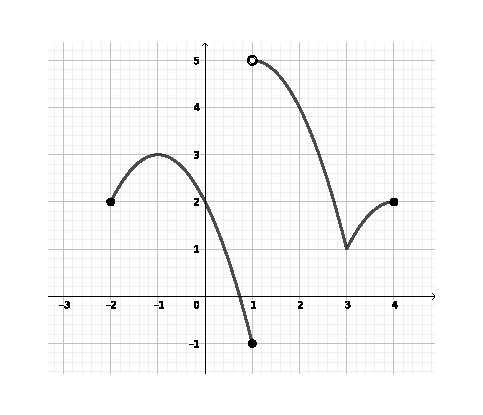
\includegraphics[width=0.6\textwidth]{TT3_fig1}
 \end{center}
 
 
 \begin{enumerate}
 \item What is the absolute maximum of $f$?\\
 (Give both $x$ and $y$ coordinates)
 
 \medskip
 
 The absolute maximum does not exist: the graph approaches $y=5$ as $x\to 1^+$, but never reaches this value.
 
 \medskip
 
 \item What is the absolute minimum of $f$?\\
  (Give both $x$ and $y$ coordinates)

\medskip

The absolute minimum value is $-1=f(1)$; i.e. it occurs at the point $(1,-1)$.

\medskip

\item At what $x$ coordinate(s) is $f'(x)=0$?

\medskip

The local maximum at $(-1,3)$ has a horizontal tangent, so $f(-1)=0$.

Note: one could argue that at the right endpoint, the value of the derivative is approaching zero. You will receive full credit whether or not you included $x=4$ as a location where $f'(x)=0$.

\medskip

\item At what $x$ coordinate(s) does $f'(x)$ not exist?

\medskip

The derivative does not exist at $x=1$, since the function is not continuous at this point. The derivative also does not exist at $x=3$ since there is a cusp at this point: the value of $f'(x)$ as $x\to 3^-$ does not match the value of $f'(x)$ as $x\to 3^+$.
\end{enumerate}


\newpage


\item (Extra group question!) \points{2}
\begin{multicols}{2}
The curve shown to the right is called the \textbf{Tschirnhausen Cubic}, and is given by the equation
\[
y^2=x^3+3x^2.
\]
From the graph, we can see that the curve has two horizontal tangents, and one vertical tangent. Determine the points at which they occur.

\begin{center}
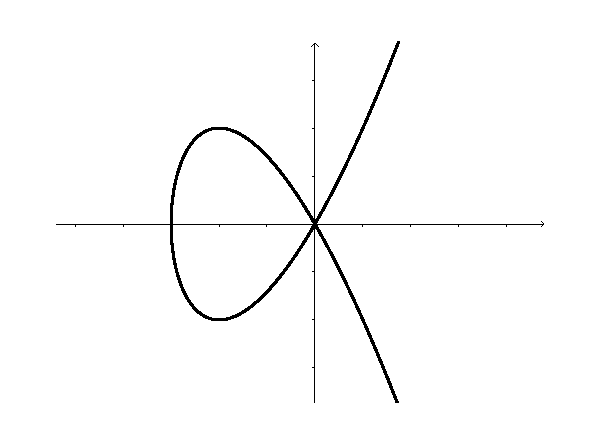
\includegraphics[width=\columnwidth]{TT3_fig2}
\end{center}
\end{multicols}

Taking the derivative of both sides using implicit differentiation, we get
\[
2y\cdot y' = 3x^2+6x, \text{ so } y' = \frac{3x^2+6x}{2y} = \frac{3x(x+2)}{2y}.
\]

We see that the numerator vanishes when $x=0$ or $x=-2$. However, at $x=0$, we have $y^2 = 0^3+3(0)^2 = 0$, so $y=0$, and the derivative is undefined at $(0,0)$, since the denominator is also zero.

(It should not be surprising that $y'$ is indeterminate at the origin: the curve intersects itself there, so there are two tangent lines!)

If $x=-2$, then $y'=0$, so we expect a horizontal tangent. Putting $x=2$ into the original equation, we find
\[
y^2 = (-2)^3+3(-2)^2 = -8+12 = 4,
\]
so $y=\pm 2$. Thus, there are horizontal tangents at $(-2,2)$ and $(-2,-2)$ as can be seen from the graph. 

For a vertical tangent, we look for a point where $y=0$ (so that $y'$ is undefined) but not the point $(0,0)$, which we have already considered. In the original equation, $y=0$ gives us
\[
0=x^3+3x^2 = x^2(x+3),
\]
so $x=0$ (which we have already ruled out), or $x=-3$. Thus, we expect that there should be a vertical tangent at $(-3,0)$, which again agrees with the graph.

\bigskip

\textbf{Note:} If you took the square root of both sides, remember that there are two solutions: $y=\pm \sqrt{x^3+3x^2}$. One corresponds to the part of the curve above the $x$-axis, the other, to the part that's below. Notice that both curves then have a cusp at the origin, so the derivative is undefined at that point: there is no tangent line at all, neither horizontal nor vertical.
\end{enumerate}
\end{document}